% Created by tikzDevice version 0.7.0 on 2014-07-01 17:48:11
% !TEX encoding = UTF-8 Unicode
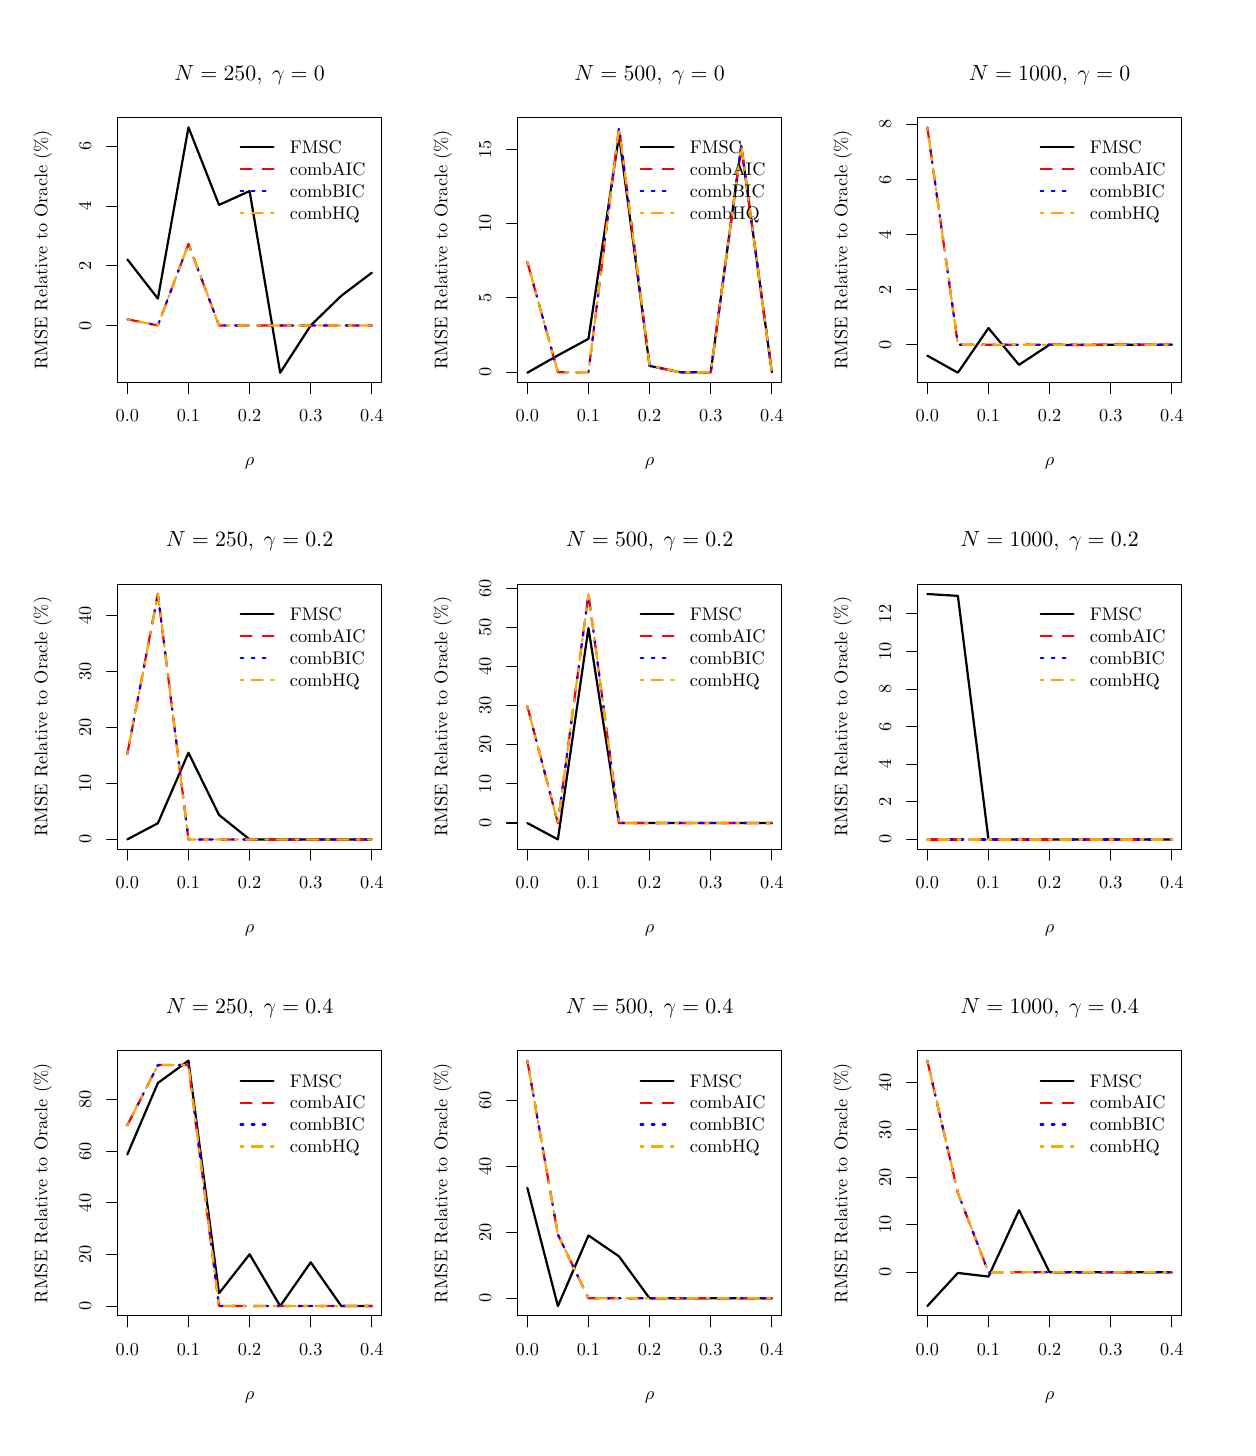
\begin{tikzpicture}[x=1pt,y=1pt]
\definecolor[named]{fillColor}{rgb}{1.00,1.00,1.00}
\path[use as bounding box,fill=fillColor,fill opacity=0.00] (0,0) rectangle (433.62,505.89);
\begin{scope}
\path[clip] ( 32.47,377.65) rectangle (127.91,473.42);
\definecolor[named]{drawColor}{rgb}{0.00,0.00,0.00}

\path[draw=drawColor,line width= 0.8pt,line join=round,line cap=round] ( 36.01,422.16) --
	( 47.05,407.97) --
	( 58.10,469.87) --
	( 69.14,441.84) --
	( 80.19,446.84) --
	( 91.24,381.20) --
	(102.28,398.28) --
	(113.33,409.00) --
	(124.37,417.34);
\end{scope}
\begin{scope}
\path[clip] (  0.00,  0.00) rectangle (433.62,505.89);
\definecolor[named]{drawColor}{rgb}{0.00,0.00,0.00}

\path[draw=drawColor,line width= 0.4pt,line join=round,line cap=round] ( 36.01,377.65) -- (124.37,377.65);

\path[draw=drawColor,line width= 0.4pt,line join=round,line cap=round] ( 36.01,377.65) -- ( 36.01,373.69);

\path[draw=drawColor,line width= 0.4pt,line join=round,line cap=round] ( 58.10,377.65) -- ( 58.10,373.69);

\path[draw=drawColor,line width= 0.4pt,line join=round,line cap=round] ( 80.19,377.65) -- ( 80.19,373.69);

\path[draw=drawColor,line width= 0.4pt,line join=round,line cap=round] (102.28,377.65) -- (102.28,373.69);

\path[draw=drawColor,line width= 0.4pt,line join=round,line cap=round] (124.37,377.65) -- (124.37,373.69);

\node[text=drawColor,anchor=base,inner sep=0pt, outer sep=0pt, scale=  0.66] at ( 36.01,363.40) {0.0};

\node[text=drawColor,anchor=base,inner sep=0pt, outer sep=0pt, scale=  0.66] at ( 58.10,363.40) {0.1};

\node[text=drawColor,anchor=base,inner sep=0pt, outer sep=0pt, scale=  0.66] at ( 80.19,363.40) {0.2};

\node[text=drawColor,anchor=base,inner sep=0pt, outer sep=0pt, scale=  0.66] at (102.28,363.40) {0.3};

\node[text=drawColor,anchor=base,inner sep=0pt, outer sep=0pt, scale=  0.66] at (124.37,363.40) {0.4};

\path[draw=drawColor,line width= 0.4pt,line join=round,line cap=round] ( 32.47,398.28) -- ( 32.47,462.98);

\path[draw=drawColor,line width= 0.4pt,line join=round,line cap=round] ( 32.47,398.28) -- ( 28.51,398.28);

\path[draw=drawColor,line width= 0.4pt,line join=round,line cap=round] ( 32.47,419.85) -- ( 28.51,419.85);

\path[draw=drawColor,line width= 0.4pt,line join=round,line cap=round] ( 32.47,441.42) -- ( 28.51,441.42);

\path[draw=drawColor,line width= 0.4pt,line join=round,line cap=round] ( 32.47,462.98) -- ( 28.51,462.98);

\node[text=drawColor,rotate= 90.00,anchor=base,inner sep=0pt, outer sep=0pt, scale=  0.66] at ( 22.97,398.28) {0};

\node[text=drawColor,rotate= 90.00,anchor=base,inner sep=0pt, outer sep=0pt, scale=  0.66] at ( 22.97,419.85) {2};

\node[text=drawColor,rotate= 90.00,anchor=base,inner sep=0pt, outer sep=0pt, scale=  0.66] at ( 22.97,441.42) {4};

\node[text=drawColor,rotate= 90.00,anchor=base,inner sep=0pt, outer sep=0pt, scale=  0.66] at ( 22.97,462.98) {6};

\path[draw=drawColor,line width= 0.4pt,line join=round,line cap=round] ( 32.47,377.65) --
	(127.91,377.65) --
	(127.91,473.42) --
	( 32.47,473.42) --
	( 32.47,377.65);
\end{scope}
\begin{scope}
\path[clip] (  0.00,337.26) rectangle (144.54,505.89);
\definecolor[named]{drawColor}{rgb}{0.00,0.00,0.00}

\node[text=drawColor,anchor=base,inner sep=0pt, outer sep=0pt, scale=  0.79] at ( 80.19,486.92) {\bfseries $N=250, \;\gamma=0$};

\node[text=drawColor,anchor=base,inner sep=0pt, outer sep=0pt, scale=  0.66] at ( 80.19,347.56) {$\rho$};

\node[text=drawColor,rotate= 90.00,anchor=base,inner sep=0pt, outer sep=0pt, scale=  0.66] at (  7.13,425.53) {RMSE Relative to Oracle (\%)};
\end{scope}
\begin{scope}
\path[clip] ( 32.47,377.65) rectangle (127.91,473.42);
\definecolor[named]{drawColor}{rgb}{1.00,0.00,0.00}

\path[draw=drawColor,line width= 0.8pt,dash pattern=on 4pt off 4pt ,line join=round,line cap=round] ( 36.01,400.52) --
	( 47.05,398.28) --
	( 58.10,427.73) --
	( 69.14,398.28) --
	( 80.19,398.28) --
	( 91.24,398.28) --
	(102.28,398.28) --
	(113.33,398.28) --
	(124.37,398.28);
\definecolor[named]{drawColor}{rgb}{0.00,0.00,1.00}

\path[draw=drawColor,line width= 0.8pt,dash pattern=on 1pt off 3pt ,line join=round,line cap=round] ( 36.01,400.52) --
	( 47.05,398.28) --
	( 58.10,427.73) --
	( 69.14,398.28) --
	( 80.19,398.28) --
	( 91.24,398.28) --
	(102.28,398.28) --
	(113.33,398.28) --
	(124.37,398.28);
\definecolor[named]{drawColor}{rgb}{1.00,0.65,0.00}

\path[draw=drawColor,line width= 0.8pt,dash pattern=on 1pt off 3pt on 4pt off 3pt ,line join=round,line cap=round] ( 36.01,400.52) --
	( 47.05,398.28) --
	( 58.10,427.73) --
	( 69.14,398.28) --
	( 80.19,398.28) --
	( 91.24,398.28) --
	(102.28,398.28) --
	(113.33,398.28) --
	(124.37,398.28);
\definecolor[named]{drawColor}{rgb}{0.00,0.00,0.00}

\path[draw=drawColor,line width= 0.8pt,line join=round,line cap=round] ( 76.94,462.63) -- ( 88.82,462.63);
\definecolor[named]{drawColor}{rgb}{1.00,0.00,0.00}

\path[draw=drawColor,line width= 0.8pt,dash pattern=on 4pt off 4pt ,line join=round,line cap=round] ( 76.94,454.71) -- ( 88.82,454.71);
\definecolor[named]{drawColor}{rgb}{0.00,0.00,1.00}

\path[draw=drawColor,line width= 0.8pt,dash pattern=on 1pt off 3pt ,line join=round,line cap=round] ( 76.94,446.79) -- ( 88.82,446.79);
\definecolor[named]{drawColor}{rgb}{1.00,0.65,0.00}

\path[draw=drawColor,line width= 0.8pt,dash pattern=on 1pt off 3pt on 4pt off 3pt ,line join=round,line cap=round] ( 76.94,438.87) -- ( 88.82,438.87);
\definecolor[named]{drawColor}{rgb}{0.00,0.00,0.00}

\node[text=drawColor,anchor=base west,inner sep=0pt, outer sep=0pt, scale=  0.66] at ( 94.76,460.35) {FMSC};

\node[text=drawColor,anchor=base west,inner sep=0pt, outer sep=0pt, scale=  0.66] at ( 94.76,452.43) {combAIC};

\node[text=drawColor,anchor=base west,inner sep=0pt, outer sep=0pt, scale=  0.66] at ( 94.76,444.51) {combBIC};

\node[text=drawColor,anchor=base west,inner sep=0pt, outer sep=0pt, scale=  0.66] at ( 94.76,436.59) {combHQ};
\end{scope}
\begin{scope}
\path[clip] (177.01,377.65) rectangle (272.45,473.42);
\definecolor[named]{drawColor}{rgb}{0.00,0.00,0.00}

\path[draw=drawColor,line width= 0.8pt,line join=round,line cap=round] (180.55,381.20) --
	(191.59,387.46) --
	(202.64,393.46) --
	(213.68,466.94) --
	(224.73,383.67) --
	(235.78,381.37) --
	(246.82,381.37) --
	(257.87,463.11) --
	(268.91,381.37);
\end{scope}
\begin{scope}
\path[clip] (  0.00,  0.00) rectangle (433.62,505.89);
\definecolor[named]{drawColor}{rgb}{0.00,0.00,0.00}

\path[draw=drawColor,line width= 0.4pt,line join=round,line cap=round] (180.55,377.65) -- (268.91,377.65);

\path[draw=drawColor,line width= 0.4pt,line join=round,line cap=round] (180.55,377.65) -- (180.55,373.69);

\path[draw=drawColor,line width= 0.4pt,line join=round,line cap=round] (202.64,377.65) -- (202.64,373.69);

\path[draw=drawColor,line width= 0.4pt,line join=round,line cap=round] (224.73,377.65) -- (224.73,373.69);

\path[draw=drawColor,line width= 0.4pt,line join=round,line cap=round] (246.82,377.65) -- (246.82,373.69);

\path[draw=drawColor,line width= 0.4pt,line join=round,line cap=round] (268.91,377.65) -- (268.91,373.69);

\node[text=drawColor,anchor=base,inner sep=0pt, outer sep=0pt, scale=  0.66] at (180.55,363.40) {0.0};

\node[text=drawColor,anchor=base,inner sep=0pt, outer sep=0pt, scale=  0.66] at (202.64,363.40) {0.1};

\node[text=drawColor,anchor=base,inner sep=0pt, outer sep=0pt, scale=  0.66] at (224.73,363.40) {0.2};

\node[text=drawColor,anchor=base,inner sep=0pt, outer sep=0pt, scale=  0.66] at (246.82,363.40) {0.3};

\node[text=drawColor,anchor=base,inner sep=0pt, outer sep=0pt, scale=  0.66] at (268.91,363.40) {0.4};

\path[draw=drawColor,line width= 0.4pt,line join=round,line cap=round] (177.01,381.37) -- (177.01,461.96);

\path[draw=drawColor,line width= 0.4pt,line join=round,line cap=round] (177.01,381.37) -- (173.05,381.37);

\path[draw=drawColor,line width= 0.4pt,line join=round,line cap=round] (177.01,408.24) -- (173.05,408.24);

\path[draw=drawColor,line width= 0.4pt,line join=round,line cap=round] (177.01,435.10) -- (173.05,435.10);

\path[draw=drawColor,line width= 0.4pt,line join=round,line cap=round] (177.01,461.96) -- (173.05,461.96);

\node[text=drawColor,rotate= 90.00,anchor=base,inner sep=0pt, outer sep=0pt, scale=  0.66] at (167.51,381.37) {0};

\node[text=drawColor,rotate= 90.00,anchor=base,inner sep=0pt, outer sep=0pt, scale=  0.66] at (167.51,408.24) {5};

\node[text=drawColor,rotate= 90.00,anchor=base,inner sep=0pt, outer sep=0pt, scale=  0.66] at (167.51,435.10) {10};

\node[text=drawColor,rotate= 90.00,anchor=base,inner sep=0pt, outer sep=0pt, scale=  0.66] at (167.51,461.96) {15};

\path[draw=drawColor,line width= 0.4pt,line join=round,line cap=round] (177.01,377.65) --
	(272.45,377.65) --
	(272.45,473.42) --
	(177.01,473.42) --
	(177.01,377.65);
\end{scope}
\begin{scope}
\path[clip] (144.54,337.26) rectangle (289.08,505.89);
\definecolor[named]{drawColor}{rgb}{0.00,0.00,0.00}

\node[text=drawColor,anchor=base,inner sep=0pt, outer sep=0pt, scale=  0.79] at (224.73,486.92) {\bfseries $N=500, \;\gamma=0$};

\node[text=drawColor,anchor=base,inner sep=0pt, outer sep=0pt, scale=  0.66] at (224.73,347.56) {$\rho$};

\node[text=drawColor,rotate= 90.00,anchor=base,inner sep=0pt, outer sep=0pt, scale=  0.66] at (151.67,425.53) {RMSE Relative to Oracle (\%)};
\end{scope}
\begin{scope}
\path[clip] (177.01,377.65) rectangle (272.45,473.42);
\definecolor[named]{drawColor}{rgb}{1.00,0.00,0.00}

\path[draw=drawColor,line width= 0.8pt,dash pattern=on 4pt off 4pt ,line join=round,line cap=round] (180.55,421.19) --
	(191.59,381.37) --
	(202.64,381.37) --
	(213.68,469.87) --
	(224.73,383.72) --
	(235.78,381.37) --
	(246.82,381.37) --
	(257.87,463.11) --
	(268.91,381.37);
\definecolor[named]{drawColor}{rgb}{0.00,0.00,1.00}

\path[draw=drawColor,line width= 0.8pt,dash pattern=on 1pt off 3pt ,line join=round,line cap=round] (180.55,421.19) --
	(191.59,381.37) --
	(202.64,381.37) --
	(213.68,469.87) --
	(224.73,383.72) --
	(235.78,381.37) --
	(246.82,381.37) --
	(257.87,463.11) --
	(268.91,381.37);
\definecolor[named]{drawColor}{rgb}{1.00,0.65,0.00}

\path[draw=drawColor,line width= 0.8pt,dash pattern=on 1pt off 3pt on 4pt off 3pt ,line join=round,line cap=round] (180.55,421.19) --
	(191.59,381.37) --
	(202.64,381.37) --
	(213.68,469.87) --
	(224.73,383.72) --
	(235.78,381.37) --
	(246.82,381.37) --
	(257.87,463.11) --
	(268.91,381.37);
\definecolor[named]{drawColor}{rgb}{0.00,0.00,0.00}

\path[draw=drawColor,line width= 0.8pt,line join=round,line cap=round] (221.48,462.63) -- (233.36,462.63);
\definecolor[named]{drawColor}{rgb}{1.00,0.00,0.00}

\path[draw=drawColor,line width= 0.8pt,dash pattern=on 4pt off 4pt ,line join=round,line cap=round] (221.48,454.71) -- (233.36,454.71);
\definecolor[named]{drawColor}{rgb}{0.00,0.00,1.00}

\path[draw=drawColor,line width= 0.8pt,dash pattern=on 1pt off 3pt ,line join=round,line cap=round] (221.48,446.79) -- (233.36,446.79);
\definecolor[named]{drawColor}{rgb}{1.00,0.65,0.00}

\path[draw=drawColor,line width= 0.8pt,dash pattern=on 1pt off 3pt on 4pt off 3pt ,line join=round,line cap=round] (221.48,438.87) -- (233.36,438.87);
\definecolor[named]{drawColor}{rgb}{0.00,0.00,0.00}

\node[text=drawColor,anchor=base west,inner sep=0pt, outer sep=0pt, scale=  0.66] at (239.30,460.35) {FMSC};

\node[text=drawColor,anchor=base west,inner sep=0pt, outer sep=0pt, scale=  0.66] at (239.30,452.43) {combAIC};

\node[text=drawColor,anchor=base west,inner sep=0pt, outer sep=0pt, scale=  0.66] at (239.30,444.51) {combBIC};

\node[text=drawColor,anchor=base west,inner sep=0pt, outer sep=0pt, scale=  0.66] at (239.30,436.59) {combHQ};
\end{scope}
\begin{scope}
\path[clip] (321.55,377.65) rectangle (416.99,473.42);
\definecolor[named]{drawColor}{rgb}{0.00,0.00,0.00}

\path[draw=drawColor,line width= 0.8pt,line join=round,line cap=round] (325.09,387.36) --
	(336.13,381.20) --
	(347.18,397.33) --
	(358.22,384.05) --
	(369.27,391.34) --
	(380.32,391.17) --
	(391.36,391.34) --
	(402.41,391.34) --
	(413.45,391.34);
\end{scope}
\begin{scope}
\path[clip] (  0.00,  0.00) rectangle (433.62,505.89);
\definecolor[named]{drawColor}{rgb}{0.00,0.00,0.00}

\path[draw=drawColor,line width= 0.4pt,line join=round,line cap=round] (325.09,377.65) -- (413.45,377.65);

\path[draw=drawColor,line width= 0.4pt,line join=round,line cap=round] (325.09,377.65) -- (325.09,373.69);

\path[draw=drawColor,line width= 0.4pt,line join=round,line cap=round] (347.18,377.65) -- (347.18,373.69);

\path[draw=drawColor,line width= 0.4pt,line join=round,line cap=round] (369.27,377.65) -- (369.27,373.69);

\path[draw=drawColor,line width= 0.4pt,line join=round,line cap=round] (391.36,377.65) -- (391.36,373.69);

\path[draw=drawColor,line width= 0.4pt,line join=round,line cap=round] (413.45,377.65) -- (413.45,373.69);

\node[text=drawColor,anchor=base,inner sep=0pt, outer sep=0pt, scale=  0.66] at (325.09,363.40) {0.0};

\node[text=drawColor,anchor=base,inner sep=0pt, outer sep=0pt, scale=  0.66] at (347.18,363.40) {0.1};

\node[text=drawColor,anchor=base,inner sep=0pt, outer sep=0pt, scale=  0.66] at (369.27,363.40) {0.2};

\node[text=drawColor,anchor=base,inner sep=0pt, outer sep=0pt, scale=  0.66] at (391.36,363.40) {0.3};

\node[text=drawColor,anchor=base,inner sep=0pt, outer sep=0pt, scale=  0.66] at (413.45,363.40) {0.4};

\path[draw=drawColor,line width= 0.4pt,line join=round,line cap=round] (321.55,391.34) -- (321.55,470.96);

\path[draw=drawColor,line width= 0.4pt,line join=round,line cap=round] (321.55,391.34) -- (317.59,391.34);

\path[draw=drawColor,line width= 0.4pt,line join=round,line cap=round] (321.55,411.24) -- (317.59,411.24);

\path[draw=drawColor,line width= 0.4pt,line join=round,line cap=round] (321.55,431.15) -- (317.59,431.15);

\path[draw=drawColor,line width= 0.4pt,line join=round,line cap=round] (321.55,451.05) -- (317.59,451.05);

\path[draw=drawColor,line width= 0.4pt,line join=round,line cap=round] (321.55,470.96) -- (317.59,470.96);

\node[text=drawColor,rotate= 90.00,anchor=base,inner sep=0pt, outer sep=0pt, scale=  0.66] at (312.05,391.34) {0};

\node[text=drawColor,rotate= 90.00,anchor=base,inner sep=0pt, outer sep=0pt, scale=  0.66] at (312.05,411.24) {2};

\node[text=drawColor,rotate= 90.00,anchor=base,inner sep=0pt, outer sep=0pt, scale=  0.66] at (312.05,431.15) {4};

\node[text=drawColor,rotate= 90.00,anchor=base,inner sep=0pt, outer sep=0pt, scale=  0.66] at (312.05,451.05) {6};

\node[text=drawColor,rotate= 90.00,anchor=base,inner sep=0pt, outer sep=0pt, scale=  0.66] at (312.05,470.96) {8};

\path[draw=drawColor,line width= 0.4pt,line join=round,line cap=round] (321.55,377.65) --
	(416.99,377.65) --
	(416.99,473.42) --
	(321.55,473.42) --
	(321.55,377.65);
\end{scope}
\begin{scope}
\path[clip] (289.08,337.26) rectangle (433.62,505.89);
\definecolor[named]{drawColor}{rgb}{0.00,0.00,0.00}

\node[text=drawColor,anchor=base,inner sep=0pt, outer sep=0pt, scale=  0.79] at (369.27,486.92) {\bfseries $N=1000, \;\gamma=0$};

\node[text=drawColor,anchor=base,inner sep=0pt, outer sep=0pt, scale=  0.66] at (369.27,347.56) {$\rho$};

\node[text=drawColor,rotate= 90.00,anchor=base,inner sep=0pt, outer sep=0pt, scale=  0.66] at (296.21,425.53) {RMSE Relative to Oracle (\%)};
\end{scope}
\begin{scope}
\path[clip] (321.55,377.65) rectangle (416.99,473.42);
\definecolor[named]{drawColor}{rgb}{1.00,0.00,0.00}

\path[draw=drawColor,line width= 0.8pt,dash pattern=on 4pt off 4pt ,line join=round,line cap=round] (325.09,469.87) --
	(336.13,391.34) --
	(347.18,391.34) --
	(358.22,391.34) --
	(369.27,391.34) --
	(380.32,391.34) --
	(391.36,391.34) --
	(402.41,391.34) --
	(413.45,391.34);
\definecolor[named]{drawColor}{rgb}{0.00,0.00,1.00}

\path[draw=drawColor,line width= 0.8pt,dash pattern=on 1pt off 3pt ,line join=round,line cap=round] (325.09,469.87) --
	(336.13,391.34) --
	(347.18,391.34) --
	(358.22,391.34) --
	(369.27,391.34) --
	(380.32,391.34) --
	(391.36,391.34) --
	(402.41,391.34) --
	(413.45,391.34);
\definecolor[named]{drawColor}{rgb}{1.00,0.65,0.00}

\path[draw=drawColor,line width= 0.8pt,dash pattern=on 1pt off 3pt on 4pt off 3pt ,line join=round,line cap=round] (325.09,469.87) --
	(336.13,391.34) --
	(347.18,391.34) --
	(358.22,391.34) --
	(369.27,391.34) --
	(380.32,391.34) --
	(391.36,391.34) --
	(402.41,391.34) --
	(413.45,391.34);
\definecolor[named]{drawColor}{rgb}{0.00,0.00,0.00}

\path[draw=drawColor,line width= 0.8pt,line join=round,line cap=round] (366.02,462.63) -- (377.90,462.63);
\definecolor[named]{drawColor}{rgb}{1.00,0.00,0.00}

\path[draw=drawColor,line width= 0.8pt,dash pattern=on 4pt off 4pt ,line join=round,line cap=round] (366.02,454.71) -- (377.90,454.71);
\definecolor[named]{drawColor}{rgb}{0.00,0.00,1.00}

\path[draw=drawColor,line width= 0.8pt,dash pattern=on 1pt off 3pt ,line join=round,line cap=round] (366.02,446.79) -- (377.90,446.79);
\definecolor[named]{drawColor}{rgb}{1.00,0.65,0.00}

\path[draw=drawColor,line width= 0.8pt,dash pattern=on 1pt off 3pt on 4pt off 3pt ,line join=round,line cap=round] (366.02,438.87) -- (377.90,438.87);
\definecolor[named]{drawColor}{rgb}{0.00,0.00,0.00}

\node[text=drawColor,anchor=base west,inner sep=0pt, outer sep=0pt, scale=  0.66] at (383.84,460.35) {FMSC};

\node[text=drawColor,anchor=base west,inner sep=0pt, outer sep=0pt, scale=  0.66] at (383.84,452.43) {combAIC};

\node[text=drawColor,anchor=base west,inner sep=0pt, outer sep=0pt, scale=  0.66] at (383.84,444.51) {combBIC};

\node[text=drawColor,anchor=base west,inner sep=0pt, outer sep=0pt, scale=  0.66] at (383.84,436.59) {combHQ};
\end{scope}
\begin{scope}
\path[clip] ( 32.47,209.02) rectangle (127.91,304.79);
\definecolor[named]{drawColor}{rgb}{0.00,0.00,0.00}

\path[draw=drawColor,line width= 0.8pt,line join=round,line cap=round] ( 36.01,212.57) --
	( 47.05,218.40) --
	( 58.10,243.88) --
	( 69.14,221.41) --
	( 80.19,212.57) --
	( 91.24,212.57) --
	(102.28,212.57) --
	(113.33,212.57) --
	(124.37,212.57);
\end{scope}
\begin{scope}
\path[clip] (  0.00,  0.00) rectangle (433.62,505.89);
\definecolor[named]{drawColor}{rgb}{0.00,0.00,0.00}

\path[draw=drawColor,line width= 0.4pt,line join=round,line cap=round] ( 36.01,209.02) -- (124.37,209.02);

\path[draw=drawColor,line width= 0.4pt,line join=round,line cap=round] ( 36.01,209.02) -- ( 36.01,205.06);

\path[draw=drawColor,line width= 0.4pt,line join=round,line cap=round] ( 58.10,209.02) -- ( 58.10,205.06);

\path[draw=drawColor,line width= 0.4pt,line join=round,line cap=round] ( 80.19,209.02) -- ( 80.19,205.06);

\path[draw=drawColor,line width= 0.4pt,line join=round,line cap=round] (102.28,209.02) -- (102.28,205.06);

\path[draw=drawColor,line width= 0.4pt,line join=round,line cap=round] (124.37,209.02) -- (124.37,205.06);

\node[text=drawColor,anchor=base,inner sep=0pt, outer sep=0pt, scale=  0.66] at ( 36.01,194.77) {0.0};

\node[text=drawColor,anchor=base,inner sep=0pt, outer sep=0pt, scale=  0.66] at ( 58.10,194.77) {0.1};

\node[text=drawColor,anchor=base,inner sep=0pt, outer sep=0pt, scale=  0.66] at ( 80.19,194.77) {0.2};

\node[text=drawColor,anchor=base,inner sep=0pt, outer sep=0pt, scale=  0.66] at (102.28,194.77) {0.3};

\node[text=drawColor,anchor=base,inner sep=0pt, outer sep=0pt, scale=  0.66] at (124.37,194.77) {0.4};

\path[draw=drawColor,line width= 0.4pt,line join=round,line cap=round] ( 32.47,212.57) -- ( 32.47,293.51);

\path[draw=drawColor,line width= 0.4pt,line join=round,line cap=round] ( 32.47,212.57) -- ( 28.51,212.57);

\path[draw=drawColor,line width= 0.4pt,line join=round,line cap=round] ( 32.47,232.80) -- ( 28.51,232.80);

\path[draw=drawColor,line width= 0.4pt,line join=round,line cap=round] ( 32.47,253.04) -- ( 28.51,253.04);

\path[draw=drawColor,line width= 0.4pt,line join=round,line cap=round] ( 32.47,273.27) -- ( 28.51,273.27);

\path[draw=drawColor,line width= 0.4pt,line join=round,line cap=round] ( 32.47,293.51) -- ( 28.51,293.51);

\node[text=drawColor,rotate= 90.00,anchor=base,inner sep=0pt, outer sep=0pt, scale=  0.66] at ( 22.97,212.57) {0};

\node[text=drawColor,rotate= 90.00,anchor=base,inner sep=0pt, outer sep=0pt, scale=  0.66] at ( 22.97,232.80) {10};

\node[text=drawColor,rotate= 90.00,anchor=base,inner sep=0pt, outer sep=0pt, scale=  0.66] at ( 22.97,253.04) {20};

\node[text=drawColor,rotate= 90.00,anchor=base,inner sep=0pt, outer sep=0pt, scale=  0.66] at ( 22.97,273.27) {30};

\node[text=drawColor,rotate= 90.00,anchor=base,inner sep=0pt, outer sep=0pt, scale=  0.66] at ( 22.97,293.51) {40};

\path[draw=drawColor,line width= 0.4pt,line join=round,line cap=round] ( 32.47,209.02) --
	(127.91,209.02) --
	(127.91,304.79) --
	( 32.47,304.79) --
	( 32.47,209.02);
\end{scope}
\begin{scope}
\path[clip] (  0.00,168.63) rectangle (144.54,337.26);
\definecolor[named]{drawColor}{rgb}{0.00,0.00,0.00}

\node[text=drawColor,anchor=base,inner sep=0pt, outer sep=0pt, scale=  0.79] at ( 80.19,318.29) {\bfseries $N=250, \;\gamma=0.2$};

\node[text=drawColor,anchor=base,inner sep=0pt, outer sep=0pt, scale=  0.66] at ( 80.19,178.93) {$\rho$};

\node[text=drawColor,rotate= 90.00,anchor=base,inner sep=0pt, outer sep=0pt, scale=  0.66] at (  7.13,256.90) {RMSE Relative to Oracle (\%)};
\end{scope}
\begin{scope}
\path[clip] ( 32.47,209.02) rectangle (127.91,304.79);
\definecolor[named]{drawColor}{rgb}{1.00,0.00,0.00}

\path[draw=drawColor,line width= 0.8pt,dash pattern=on 4pt off 4pt ,line join=round,line cap=round] ( 36.01,243.45) --
	( 47.05,301.24) --
	( 58.10,212.57) --
	( 69.14,212.57) --
	( 80.19,212.57) --
	( 91.24,212.57) --
	(102.28,212.57) --
	(113.33,212.57) --
	(124.37,212.57);
\definecolor[named]{drawColor}{rgb}{0.00,0.00,1.00}

\path[draw=drawColor,line width= 0.8pt,dash pattern=on 1pt off 3pt ,line join=round,line cap=round] ( 36.01,243.45) --
	( 47.05,301.24) --
	( 58.10,212.57) --
	( 69.14,212.57) --
	( 80.19,212.57) --
	( 91.24,212.57) --
	(102.28,212.57) --
	(113.33,212.57) --
	(124.37,212.57);
\definecolor[named]{drawColor}{rgb}{1.00,0.65,0.00}

\path[draw=drawColor,line width= 0.8pt,dash pattern=on 1pt off 3pt on 4pt off 3pt ,line join=round,line cap=round] ( 36.01,243.45) --
	( 47.05,301.24) --
	( 58.10,212.57) --
	( 69.14,212.57) --
	( 80.19,212.57) --
	( 91.24,212.57) --
	(102.28,212.57) --
	(113.33,212.57) --
	(124.37,212.57);
\definecolor[named]{drawColor}{rgb}{0.00,0.00,0.00}

\path[draw=drawColor,line width= 0.8pt,line join=round,line cap=round] ( 76.94,294.00) -- ( 88.82,294.00);
\definecolor[named]{drawColor}{rgb}{1.00,0.00,0.00}

\path[draw=drawColor,line width= 0.8pt,dash pattern=on 4pt off 4pt ,line join=round,line cap=round] ( 76.94,286.08) -- ( 88.82,286.08);
\definecolor[named]{drawColor}{rgb}{0.00,0.00,1.00}

\path[draw=drawColor,line width= 0.8pt,dash pattern=on 1pt off 3pt ,line join=round,line cap=round] ( 76.94,278.16) -- ( 88.82,278.16);
\definecolor[named]{drawColor}{rgb}{1.00,0.65,0.00}

\path[draw=drawColor,line width= 0.8pt,dash pattern=on 1pt off 3pt on 4pt off 3pt ,line join=round,line cap=round] ( 76.94,270.24) -- ( 88.82,270.24);
\definecolor[named]{drawColor}{rgb}{0.00,0.00,0.00}

\node[text=drawColor,anchor=base west,inner sep=0pt, outer sep=0pt, scale=  0.66] at ( 94.76,291.72) {FMSC};

\node[text=drawColor,anchor=base west,inner sep=0pt, outer sep=0pt, scale=  0.66] at ( 94.76,283.80) {combAIC};

\node[text=drawColor,anchor=base west,inner sep=0pt, outer sep=0pt, scale=  0.66] at ( 94.76,275.88) {combBIC};

\node[text=drawColor,anchor=base west,inner sep=0pt, outer sep=0pt, scale=  0.66] at ( 94.76,267.96) {combHQ};
\end{scope}
\begin{scope}
\path[clip] (177.01,209.02) rectangle (272.45,304.79);
\definecolor[named]{drawColor}{rgb}{0.00,0.00,0.00}

\path[draw=drawColor,line width= 0.8pt,line join=round,line cap=round] (180.55,218.48) --
	(191.59,212.57) --
	(202.64,288.94) --
	(213.68,218.48) --
	(224.73,218.48) --
	(235.78,218.48) --
	(246.82,218.48) --
	(257.87,218.48) --
	(268.91,218.48);
\end{scope}
\begin{scope}
\path[clip] (  0.00,  0.00) rectangle (433.62,505.89);
\definecolor[named]{drawColor}{rgb}{0.00,0.00,0.00}

\path[draw=drawColor,line width= 0.4pt,line join=round,line cap=round] (180.55,209.02) -- (268.91,209.02);

\path[draw=drawColor,line width= 0.4pt,line join=round,line cap=round] (180.55,209.02) -- (180.55,205.06);

\path[draw=drawColor,line width= 0.4pt,line join=round,line cap=round] (202.64,209.02) -- (202.64,205.06);

\path[draw=drawColor,line width= 0.4pt,line join=round,line cap=round] (224.73,209.02) -- (224.73,205.06);

\path[draw=drawColor,line width= 0.4pt,line join=round,line cap=round] (246.82,209.02) -- (246.82,205.06);

\path[draw=drawColor,line width= 0.4pt,line join=round,line cap=round] (268.91,209.02) -- (268.91,205.06);

\node[text=drawColor,anchor=base,inner sep=0pt, outer sep=0pt, scale=  0.66] at (180.55,194.77) {0.0};

\node[text=drawColor,anchor=base,inner sep=0pt, outer sep=0pt, scale=  0.66] at (202.64,194.77) {0.1};

\node[text=drawColor,anchor=base,inner sep=0pt, outer sep=0pt, scale=  0.66] at (224.73,194.77) {0.2};

\node[text=drawColor,anchor=base,inner sep=0pt, outer sep=0pt, scale=  0.66] at (246.82,194.77) {0.3};

\node[text=drawColor,anchor=base,inner sep=0pt, outer sep=0pt, scale=  0.66] at (268.91,194.77) {0.4};

\path[draw=drawColor,line width= 0.4pt,line join=round,line cap=round] (177.01,218.48) -- (177.01,303.34);

\path[draw=drawColor,line width= 0.4pt,line join=round,line cap=round] (177.01,218.48) -- (173.05,218.48);

\path[draw=drawColor,line width= 0.4pt,line join=round,line cap=round] (177.01,232.62) -- (173.05,232.62);

\path[draw=drawColor,line width= 0.4pt,line join=round,line cap=round] (177.01,246.77) -- (173.05,246.77);

\path[draw=drawColor,line width= 0.4pt,line join=round,line cap=round] (177.01,260.91) -- (173.05,260.91);

\path[draw=drawColor,line width= 0.4pt,line join=round,line cap=round] (177.01,275.05) -- (173.05,275.05);

\path[draw=drawColor,line width= 0.4pt,line join=round,line cap=round] (177.01,289.19) -- (173.05,289.19);

\path[draw=drawColor,line width= 0.4pt,line join=round,line cap=round] (177.01,303.34) -- (173.05,303.34);

\node[text=drawColor,rotate= 90.00,anchor=base,inner sep=0pt, outer sep=0pt, scale=  0.66] at (167.51,218.48) {0};

\node[text=drawColor,rotate= 90.00,anchor=base,inner sep=0pt, outer sep=0pt, scale=  0.66] at (167.51,232.62) {10};

\node[text=drawColor,rotate= 90.00,anchor=base,inner sep=0pt, outer sep=0pt, scale=  0.66] at (167.51,246.77) {20};

\node[text=drawColor,rotate= 90.00,anchor=base,inner sep=0pt, outer sep=0pt, scale=  0.66] at (167.51,260.91) {30};

\node[text=drawColor,rotate= 90.00,anchor=base,inner sep=0pt, outer sep=0pt, scale=  0.66] at (167.51,275.05) {40};

\node[text=drawColor,rotate= 90.00,anchor=base,inner sep=0pt, outer sep=0pt, scale=  0.66] at (167.51,289.19) {50};

\node[text=drawColor,rotate= 90.00,anchor=base,inner sep=0pt, outer sep=0pt, scale=  0.66] at (167.51,303.34) {60};

\path[draw=drawColor,line width= 0.4pt,line join=round,line cap=round] (177.01,209.02) --
	(272.45,209.02) --
	(272.45,304.79) --
	(177.01,304.79) --
	(177.01,209.02);
\end{scope}
\begin{scope}
\path[clip] (144.54,168.63) rectangle (289.08,337.26);
\definecolor[named]{drawColor}{rgb}{0.00,0.00,0.00}

\node[text=drawColor,anchor=base,inner sep=0pt, outer sep=0pt, scale=  0.79] at (224.73,318.29) {\bfseries $N=500, \;\gamma=0.2$};

\node[text=drawColor,anchor=base,inner sep=0pt, outer sep=0pt, scale=  0.66] at (224.73,178.93) {$\rho$};

\node[text=drawColor,rotate= 90.00,anchor=base,inner sep=0pt, outer sep=0pt, scale=  0.66] at (151.67,256.90) {RMSE Relative to Oracle (\%)};
\end{scope}
\begin{scope}
\path[clip] (177.01,209.02) rectangle (272.45,304.79);
\definecolor[named]{drawColor}{rgb}{1.00,0.00,0.00}

\path[draw=drawColor,line width= 0.8pt,dash pattern=on 4pt off 4pt ,line join=round,line cap=round] (180.55,260.72) --
	(191.59,218.48) --
	(202.64,301.24) --
	(213.68,218.48) --
	(224.73,218.48) --
	(235.78,218.48) --
	(246.82,218.48) --
	(257.87,218.48) --
	(268.91,218.48);
\definecolor[named]{drawColor}{rgb}{0.00,0.00,1.00}

\path[draw=drawColor,line width= 0.8pt,dash pattern=on 1pt off 3pt ,line join=round,line cap=round] (180.55,260.72) --
	(191.59,218.48) --
	(202.64,301.24) --
	(213.68,218.48) --
	(224.73,218.48) --
	(235.78,218.48) --
	(246.82,218.48) --
	(257.87,218.48) --
	(268.91,218.48);
\definecolor[named]{drawColor}{rgb}{1.00,0.65,0.00}

\path[draw=drawColor,line width= 0.8pt,dash pattern=on 1pt off 3pt on 4pt off 3pt ,line join=round,line cap=round] (180.55,260.72) --
	(191.59,218.48) --
	(202.64,301.24) --
	(213.68,218.48) --
	(224.73,218.48) --
	(235.78,218.48) --
	(246.82,218.48) --
	(257.87,218.48) --
	(268.91,218.48);
\definecolor[named]{drawColor}{rgb}{0.00,0.00,0.00}

\path[draw=drawColor,line width= 0.8pt,line join=round,line cap=round] (221.48,294.00) -- (233.36,294.00);
\definecolor[named]{drawColor}{rgb}{1.00,0.00,0.00}

\path[draw=drawColor,line width= 0.8pt,dash pattern=on 4pt off 4pt ,line join=round,line cap=round] (221.48,286.08) -- (233.36,286.08);
\definecolor[named]{drawColor}{rgb}{0.00,0.00,1.00}

\path[draw=drawColor,line width= 0.8pt,dash pattern=on 1pt off 3pt ,line join=round,line cap=round] (221.48,278.16) -- (233.36,278.16);
\definecolor[named]{drawColor}{rgb}{1.00,0.65,0.00}

\path[draw=drawColor,line width= 0.8pt,dash pattern=on 1pt off 3pt on 4pt off 3pt ,line join=round,line cap=round] (221.48,270.24) -- (233.36,270.24);
\definecolor[named]{drawColor}{rgb}{0.00,0.00,0.00}

\node[text=drawColor,anchor=base west,inner sep=0pt, outer sep=0pt, scale=  0.66] at (239.30,291.72) {FMSC};

\node[text=drawColor,anchor=base west,inner sep=0pt, outer sep=0pt, scale=  0.66] at (239.30,283.80) {combAIC};

\node[text=drawColor,anchor=base west,inner sep=0pt, outer sep=0pt, scale=  0.66] at (239.30,275.88) {combBIC};

\node[text=drawColor,anchor=base west,inner sep=0pt, outer sep=0pt, scale=  0.66] at (239.30,267.96) {combHQ};
\end{scope}
\begin{scope}
\path[clip] (321.55,209.02) rectangle (416.99,304.79);
\definecolor[named]{drawColor}{rgb}{0.00,0.00,0.00}

\path[draw=drawColor,line width= 0.8pt,line join=round,line cap=round] (325.09,301.24) --
	(336.13,300.57) --
	(347.18,212.57) --
	(358.22,212.57) --
	(369.27,212.57) --
	(380.32,212.57) --
	(391.36,212.57) --
	(402.41,212.57) --
	(413.45,212.57);
\end{scope}
\begin{scope}
\path[clip] (  0.00,  0.00) rectangle (433.62,505.89);
\definecolor[named]{drawColor}{rgb}{0.00,0.00,0.00}

\path[draw=drawColor,line width= 0.4pt,line join=round,line cap=round] (325.09,209.02) -- (413.45,209.02);

\path[draw=drawColor,line width= 0.4pt,line join=round,line cap=round] (325.09,209.02) -- (325.09,205.06);

\path[draw=drawColor,line width= 0.4pt,line join=round,line cap=round] (347.18,209.02) -- (347.18,205.06);

\path[draw=drawColor,line width= 0.4pt,line join=round,line cap=round] (369.27,209.02) -- (369.27,205.06);

\path[draw=drawColor,line width= 0.4pt,line join=round,line cap=round] (391.36,209.02) -- (391.36,205.06);

\path[draw=drawColor,line width= 0.4pt,line join=round,line cap=round] (413.45,209.02) -- (413.45,205.06);

\node[text=drawColor,anchor=base,inner sep=0pt, outer sep=0pt, scale=  0.66] at (325.09,194.77) {0.0};

\node[text=drawColor,anchor=base,inner sep=0pt, outer sep=0pt, scale=  0.66] at (347.18,194.77) {0.1};

\node[text=drawColor,anchor=base,inner sep=0pt, outer sep=0pt, scale=  0.66] at (369.27,194.77) {0.2};

\node[text=drawColor,anchor=base,inner sep=0pt, outer sep=0pt, scale=  0.66] at (391.36,194.77) {0.3};

\node[text=drawColor,anchor=base,inner sep=0pt, outer sep=0pt, scale=  0.66] at (413.45,194.77) {0.4};

\path[draw=drawColor,line width= 0.4pt,line join=round,line cap=round] (321.55,212.57) -- (321.55,294.04);

\path[draw=drawColor,line width= 0.4pt,line join=round,line cap=round] (321.55,212.57) -- (317.59,212.57);

\path[draw=drawColor,line width= 0.4pt,line join=round,line cap=round] (321.55,226.15) -- (317.59,226.15);

\path[draw=drawColor,line width= 0.4pt,line join=round,line cap=round] (321.55,239.73) -- (317.59,239.73);

\path[draw=drawColor,line width= 0.4pt,line join=round,line cap=round] (321.55,253.30) -- (317.59,253.30);

\path[draw=drawColor,line width= 0.4pt,line join=round,line cap=round] (321.55,266.88) -- (317.59,266.88);

\path[draw=drawColor,line width= 0.4pt,line join=round,line cap=round] (321.55,280.46) -- (317.59,280.46);

\path[draw=drawColor,line width= 0.4pt,line join=round,line cap=round] (321.55,294.04) -- (317.59,294.04);

\node[text=drawColor,rotate= 90.00,anchor=base,inner sep=0pt, outer sep=0pt, scale=  0.66] at (312.05,212.57) {0};

\node[text=drawColor,rotate= 90.00,anchor=base,inner sep=0pt, outer sep=0pt, scale=  0.66] at (312.05,226.15) {2};

\node[text=drawColor,rotate= 90.00,anchor=base,inner sep=0pt, outer sep=0pt, scale=  0.66] at (312.05,239.73) {4};

\node[text=drawColor,rotate= 90.00,anchor=base,inner sep=0pt, outer sep=0pt, scale=  0.66] at (312.05,253.30) {6};

\node[text=drawColor,rotate= 90.00,anchor=base,inner sep=0pt, outer sep=0pt, scale=  0.66] at (312.05,266.88) {8};

\node[text=drawColor,rotate= 90.00,anchor=base,inner sep=0pt, outer sep=0pt, scale=  0.66] at (312.05,280.46) {10};

\node[text=drawColor,rotate= 90.00,anchor=base,inner sep=0pt, outer sep=0pt, scale=  0.66] at (312.05,294.04) {12};

\path[draw=drawColor,line width= 0.4pt,line join=round,line cap=round] (321.55,209.02) --
	(416.99,209.02) --
	(416.99,304.79) --
	(321.55,304.79) --
	(321.55,209.02);
\end{scope}
\begin{scope}
\path[clip] (289.08,168.63) rectangle (433.62,337.26);
\definecolor[named]{drawColor}{rgb}{0.00,0.00,0.00}

\node[text=drawColor,anchor=base,inner sep=0pt, outer sep=0pt, scale=  0.79] at (369.27,318.29) {\bfseries $N=1000, \;\gamma=0.2$};

\node[text=drawColor,anchor=base,inner sep=0pt, outer sep=0pt, scale=  0.66] at (369.27,178.93) {$\rho$};

\node[text=drawColor,rotate= 90.00,anchor=base,inner sep=0pt, outer sep=0pt, scale=  0.66] at (296.21,256.90) {RMSE Relative to Oracle (\%)};
\end{scope}
\begin{scope}
\path[clip] (321.55,209.02) rectangle (416.99,304.79);
\definecolor[named]{drawColor}{rgb}{1.00,0.00,0.00}

\path[draw=drawColor,line width= 0.8pt,dash pattern=on 4pt off 4pt ,line join=round,line cap=round] (325.09,212.57) --
	(336.13,212.57) --
	(347.18,212.57) --
	(358.22,212.57) --
	(369.27,212.57) --
	(380.32,212.57) --
	(391.36,212.57) --
	(402.41,212.57) --
	(413.45,212.57);
\definecolor[named]{drawColor}{rgb}{0.00,0.00,1.00}

\path[draw=drawColor,line width= 0.8pt,dash pattern=on 1pt off 3pt ,line join=round,line cap=round] (325.09,212.57) --
	(336.13,212.57) --
	(347.18,212.57) --
	(358.22,212.57) --
	(369.27,212.57) --
	(380.32,212.57) --
	(391.36,212.57) --
	(402.41,212.57) --
	(413.45,212.57);
\definecolor[named]{drawColor}{rgb}{1.00,0.65,0.00}

\path[draw=drawColor,line width= 0.8pt,dash pattern=on 1pt off 3pt on 4pt off 3pt ,line join=round,line cap=round] (325.09,212.57) --
	(336.13,212.57) --
	(347.18,212.57) --
	(358.22,212.57) --
	(369.27,212.57) --
	(380.32,212.57) --
	(391.36,212.57) --
	(402.41,212.57) --
	(413.45,212.57);
\definecolor[named]{drawColor}{rgb}{0.00,0.00,0.00}

\path[draw=drawColor,line width= 0.8pt,line join=round,line cap=round] (366.02,294.00) -- (377.90,294.00);
\definecolor[named]{drawColor}{rgb}{1.00,0.00,0.00}

\path[draw=drawColor,line width= 0.8pt,dash pattern=on 4pt off 4pt ,line join=round,line cap=round] (366.02,286.08) -- (377.90,286.08);
\definecolor[named]{drawColor}{rgb}{0.00,0.00,1.00}

\path[draw=drawColor,line width= 0.8pt,dash pattern=on 1pt off 3pt ,line join=round,line cap=round] (366.02,278.16) -- (377.90,278.16);
\definecolor[named]{drawColor}{rgb}{1.00,0.65,0.00}

\path[draw=drawColor,line width= 0.8pt,dash pattern=on 1pt off 3pt on 4pt off 3pt ,line join=round,line cap=round] (366.02,270.24) -- (377.90,270.24);
\definecolor[named]{drawColor}{rgb}{0.00,0.00,0.00}

\node[text=drawColor,anchor=base west,inner sep=0pt, outer sep=0pt, scale=  0.66] at (383.84,291.72) {FMSC};

\node[text=drawColor,anchor=base west,inner sep=0pt, outer sep=0pt, scale=  0.66] at (383.84,283.80) {combAIC};

\node[text=drawColor,anchor=base west,inner sep=0pt, outer sep=0pt, scale=  0.66] at (383.84,275.88) {combBIC};

\node[text=drawColor,anchor=base west,inner sep=0pt, outer sep=0pt, scale=  0.66] at (383.84,267.96) {combHQ};
\end{scope}
\begin{scope}
\path[clip] ( 32.47, 40.39) rectangle (127.91,136.16);
\definecolor[named]{drawColor}{rgb}{0.00,0.00,0.00}

\path[draw=drawColor,line width= 0.8pt,line join=round,line cap=round] ( 36.01, 98.71) --
	( 47.05,124.55) --
	( 58.10,132.61) --
	( 69.14, 48.57) --
	( 80.19, 62.65) --
	( 91.24, 43.94) --
	(102.28, 59.75) --
	(113.33, 43.94) --
	(124.37, 43.94);
\end{scope}
\begin{scope}
\path[clip] (  0.00,  0.00) rectangle (433.62,505.89);
\definecolor[named]{drawColor}{rgb}{0.00,0.00,0.00}

\path[draw=drawColor,line width= 0.4pt,line join=round,line cap=round] ( 36.01, 40.39) -- (124.37, 40.39);

\path[draw=drawColor,line width= 0.4pt,line join=round,line cap=round] ( 36.01, 40.39) -- ( 36.01, 36.43);

\path[draw=drawColor,line width= 0.4pt,line join=round,line cap=round] ( 58.10, 40.39) -- ( 58.10, 36.43);

\path[draw=drawColor,line width= 0.4pt,line join=round,line cap=round] ( 80.19, 40.39) -- ( 80.19, 36.43);

\path[draw=drawColor,line width= 0.4pt,line join=round,line cap=round] (102.28, 40.39) -- (102.28, 36.43);

\path[draw=drawColor,line width= 0.4pt,line join=round,line cap=round] (124.37, 40.39) -- (124.37, 36.43);

\node[text=drawColor,anchor=base,inner sep=0pt, outer sep=0pt, scale=  0.66] at ( 36.01, 26.14) {0.0};

\node[text=drawColor,anchor=base,inner sep=0pt, outer sep=0pt, scale=  0.66] at ( 58.10, 26.14) {0.1};

\node[text=drawColor,anchor=base,inner sep=0pt, outer sep=0pt, scale=  0.66] at ( 80.19, 26.14) {0.2};

\node[text=drawColor,anchor=base,inner sep=0pt, outer sep=0pt, scale=  0.66] at (102.28, 26.14) {0.3};

\node[text=drawColor,anchor=base,inner sep=0pt, outer sep=0pt, scale=  0.66] at (124.37, 26.14) {0.4};

\path[draw=drawColor,line width= 0.4pt,line join=round,line cap=round] ( 32.47, 43.94) -- ( 32.47,118.53);

\path[draw=drawColor,line width= 0.4pt,line join=round,line cap=round] ( 32.47, 43.94) -- ( 28.51, 43.94);

\path[draw=drawColor,line width= 0.4pt,line join=round,line cap=round] ( 32.47, 62.59) -- ( 28.51, 62.59);

\path[draw=drawColor,line width= 0.4pt,line join=round,line cap=round] ( 32.47, 81.23) -- ( 28.51, 81.23);

\path[draw=drawColor,line width= 0.4pt,line join=round,line cap=round] ( 32.47, 99.88) -- ( 28.51, 99.88);

\path[draw=drawColor,line width= 0.4pt,line join=round,line cap=round] ( 32.47,118.53) -- ( 28.51,118.53);

\node[text=drawColor,rotate= 90.00,anchor=base,inner sep=0pt, outer sep=0pt, scale=  0.66] at ( 22.97, 43.94) {0};

\node[text=drawColor,rotate= 90.00,anchor=base,inner sep=0pt, outer sep=0pt, scale=  0.66] at ( 22.97, 62.59) {20};

\node[text=drawColor,rotate= 90.00,anchor=base,inner sep=0pt, outer sep=0pt, scale=  0.66] at ( 22.97, 81.23) {40};

\node[text=drawColor,rotate= 90.00,anchor=base,inner sep=0pt, outer sep=0pt, scale=  0.66] at ( 22.97, 99.88) {60};

\node[text=drawColor,rotate= 90.00,anchor=base,inner sep=0pt, outer sep=0pt, scale=  0.66] at ( 22.97,118.53) {80};

\path[draw=drawColor,line width= 0.4pt,line join=round,line cap=round] ( 32.47, 40.39) --
	(127.91, 40.39) --
	(127.91,136.16) --
	( 32.47,136.16) --
	( 32.47, 40.39);
\end{scope}
\begin{scope}
\path[clip] (  0.00,  0.00) rectangle (144.54,168.63);
\definecolor[named]{drawColor}{rgb}{0.00,0.00,0.00}

\node[text=drawColor,anchor=base,inner sep=0pt, outer sep=0pt, scale=  0.79] at ( 80.19,149.66) {\bfseries $N=250, \;\gamma=0.4$};

\node[text=drawColor,anchor=base,inner sep=0pt, outer sep=0pt, scale=  0.66] at ( 80.19, 10.30) {$\rho$};

\node[text=drawColor,rotate= 90.00,anchor=base,inner sep=0pt, outer sep=0pt, scale=  0.66] at (  7.13, 88.27) {RMSE Relative to Oracle (\%)};
\end{scope}
\begin{scope}
\path[clip] ( 32.47, 40.39) rectangle (127.91,136.16);
\definecolor[named]{drawColor}{rgb}{1.00,0.00,0.00}

\path[draw=drawColor,line width= 0.8pt,dash pattern=on 4pt off 4pt ,line join=round,line cap=round] ( 36.01,109.27) --
	( 47.05,131.01) --
	( 58.10,131.05) --
	( 69.14, 43.94) --
	( 80.19, 43.94) --
	( 91.24, 43.94) --
	(102.28, 43.94) --
	(113.33, 43.94) --
	(124.37, 43.94);
\definecolor[named]{drawColor}{rgb}{0.00,0.00,1.00}

\path[draw=drawColor,line width= 0.8pt,dash pattern=on 1pt off 3pt ,line join=round,line cap=round] ( 36.01,109.27) --
	( 47.05,131.01) --
	( 58.10,131.05) --
	( 69.14, 43.94) --
	( 80.19, 43.94) --
	( 91.24, 43.94) --
	(102.28, 43.94) --
	(113.33, 43.94) --
	(124.37, 43.94);
\definecolor[named]{drawColor}{rgb}{1.00,0.65,0.00}

\path[draw=drawColor,line width= 0.8pt,dash pattern=on 1pt off 3pt on 4pt off 3pt ,line join=round,line cap=round] ( 36.01,109.27) --
	( 47.05,131.01) --
	( 58.10,131.05) --
	( 69.14, 43.94) --
	( 80.19, 43.94) --
	( 91.24, 43.94) --
	(102.28, 43.94) --
	(113.33, 43.94) --
	(124.37, 43.94);
\definecolor[named]{drawColor}{rgb}{0.00,0.00,0.00}

\path[draw=drawColor,line width= 0.8pt,line join=round,line cap=round] ( 76.94,125.37) -- ( 88.82,125.37);
\definecolor[named]{drawColor}{rgb}{1.00,0.00,0.00}

\path[draw=drawColor,line width= 0.8pt,dash pattern=on 4pt off 4pt ,line join=round,line cap=round] ( 76.94,117.45) -- ( 88.82,117.45);
\definecolor[named]{drawColor}{rgb}{0.00,0.00,1.00}

\path[draw=drawColor,line width= 0.8pt,dash pattern=on 1pt off 3pt ,line join=round,line cap=round] ( 76.94,109.53) -- ( 88.82,109.53);
\definecolor[named]{drawColor}{rgb}{1.00,0.65,0.00}

\path[draw=drawColor,line width= 0.8pt,dash pattern=on 1pt off 3pt on 4pt off 3pt ,line join=round,line cap=round] ( 76.94,101.61) -- ( 88.82,101.61);
\definecolor[named]{drawColor}{rgb}{0.00,0.00,0.00}

\node[text=drawColor,anchor=base west,inner sep=0pt, outer sep=0pt, scale=  0.66] at ( 94.76,123.09) {FMSC};

\node[text=drawColor,anchor=base west,inner sep=0pt, outer sep=0pt, scale=  0.66] at ( 94.76,115.17) {combAIC};

\node[text=drawColor,anchor=base west,inner sep=0pt, outer sep=0pt, scale=  0.66] at ( 94.76,107.25) {combBIC};

\node[text=drawColor,anchor=base west,inner sep=0pt, outer sep=0pt, scale=  0.66] at ( 94.76, 99.33) {combHQ};
\end{scope}
\begin{scope}
\path[clip] (177.01, 40.39) rectangle (272.45,136.16);
\definecolor[named]{drawColor}{rgb}{0.00,0.00,0.00}

\path[draw=drawColor,line width= 0.8pt,line join=round,line cap=round] (180.55, 86.68) --
	(191.59, 43.94) --
	(202.64, 69.45) --
	(213.68, 61.89) --
	(224.73, 46.73) --
	(235.78, 46.73) --
	(246.82, 46.73) --
	(257.87, 46.73) --
	(268.91, 46.73);
\end{scope}
\begin{scope}
\path[clip] (  0.00,  0.00) rectangle (433.62,505.89);
\definecolor[named]{drawColor}{rgb}{0.00,0.00,0.00}

\path[draw=drawColor,line width= 0.4pt,line join=round,line cap=round] (180.55, 40.39) -- (268.91, 40.39);

\path[draw=drawColor,line width= 0.4pt,line join=round,line cap=round] (180.55, 40.39) -- (180.55, 36.43);

\path[draw=drawColor,line width= 0.4pt,line join=round,line cap=round] (202.64, 40.39) -- (202.64, 36.43);

\path[draw=drawColor,line width= 0.4pt,line join=round,line cap=round] (224.73, 40.39) -- (224.73, 36.43);

\path[draw=drawColor,line width= 0.4pt,line join=round,line cap=round] (246.82, 40.39) -- (246.82, 36.43);

\path[draw=drawColor,line width= 0.4pt,line join=round,line cap=round] (268.91, 40.39) -- (268.91, 36.43);

\node[text=drawColor,anchor=base,inner sep=0pt, outer sep=0pt, scale=  0.66] at (180.55, 26.14) {0.0};

\node[text=drawColor,anchor=base,inner sep=0pt, outer sep=0pt, scale=  0.66] at (202.64, 26.14) {0.1};

\node[text=drawColor,anchor=base,inner sep=0pt, outer sep=0pt, scale=  0.66] at (224.73, 26.14) {0.2};

\node[text=drawColor,anchor=base,inner sep=0pt, outer sep=0pt, scale=  0.66] at (246.82, 26.14) {0.3};

\node[text=drawColor,anchor=base,inner sep=0pt, outer sep=0pt, scale=  0.66] at (268.91, 26.14) {0.4};

\path[draw=drawColor,line width= 0.4pt,line join=round,line cap=round] (177.01, 46.73) -- (177.01,118.33);

\path[draw=drawColor,line width= 0.4pt,line join=round,line cap=round] (177.01, 46.73) -- (173.05, 46.73);

\path[draw=drawColor,line width= 0.4pt,line join=round,line cap=round] (177.01, 70.59) -- (173.05, 70.59);

\path[draw=drawColor,line width= 0.4pt,line join=round,line cap=round] (177.01, 94.46) -- (173.05, 94.46);

\path[draw=drawColor,line width= 0.4pt,line join=round,line cap=round] (177.01,118.33) -- (173.05,118.33);

\node[text=drawColor,rotate= 90.00,anchor=base,inner sep=0pt, outer sep=0pt, scale=  0.66] at (167.51, 46.73) {0};

\node[text=drawColor,rotate= 90.00,anchor=base,inner sep=0pt, outer sep=0pt, scale=  0.66] at (167.51, 70.59) {20};

\node[text=drawColor,rotate= 90.00,anchor=base,inner sep=0pt, outer sep=0pt, scale=  0.66] at (167.51, 94.46) {40};

\node[text=drawColor,rotate= 90.00,anchor=base,inner sep=0pt, outer sep=0pt, scale=  0.66] at (167.51,118.33) {60};

\path[draw=drawColor,line width= 0.4pt,line join=round,line cap=round] (177.01, 40.39) --
	(272.45, 40.39) --
	(272.45,136.16) --
	(177.01,136.16) --
	(177.01, 40.39);
\end{scope}
\begin{scope}
\path[clip] (144.54,  0.00) rectangle (289.08,168.63);
\definecolor[named]{drawColor}{rgb}{0.00,0.00,0.00}

\node[text=drawColor,anchor=base,inner sep=0pt, outer sep=0pt, scale=  0.79] at (224.73,149.66) {\bfseries $N=500, \;\gamma=0.4$};

\node[text=drawColor,anchor=base,inner sep=0pt, outer sep=0pt, scale=  0.66] at (224.73, 10.30) {$\rho$};

\node[text=drawColor,rotate= 90.00,anchor=base,inner sep=0pt, outer sep=0pt, scale=  0.66] at (151.67, 88.27) {RMSE Relative to Oracle (\%)};
\end{scope}
\begin{scope}
\path[clip] (177.01, 40.39) rectangle (272.45,136.16);
\definecolor[named]{drawColor}{rgb}{1.00,0.00,0.00}

\path[draw=drawColor,line width= 0.8pt,dash pattern=on 4pt off 4pt ,line join=round,line cap=round] (180.55,132.61) --
	(191.59, 69.80) --
	(202.64, 46.73) --
	(213.68, 46.73) --
	(224.73, 46.73) --
	(235.78, 46.73) --
	(246.82, 46.73) --
	(257.87, 46.73) --
	(268.91, 46.73);
\definecolor[named]{drawColor}{rgb}{0.00,0.00,1.00}

\path[draw=drawColor,line width= 0.8pt,dash pattern=on 1pt off 3pt ,line join=round,line cap=round] (180.55,132.61) --
	(191.59, 69.80) --
	(202.64, 46.73) --
	(213.68, 46.73) --
	(224.73, 46.73) --
	(235.78, 46.73) --
	(246.82, 46.73) --
	(257.87, 46.73) --
	(268.91, 46.73);
\definecolor[named]{drawColor}{rgb}{1.00,0.65,0.00}

\path[draw=drawColor,line width= 0.8pt,dash pattern=on 1pt off 3pt on 4pt off 3pt ,line join=round,line cap=round] (180.55,132.61) --
	(191.59, 69.80) --
	(202.64, 46.73) --
	(213.68, 46.73) --
	(224.73, 46.73) --
	(235.78, 46.73) --
	(246.82, 46.73) --
	(257.87, 46.73) --
	(268.91, 46.73);
\definecolor[named]{drawColor}{rgb}{0.00,0.00,0.00}

\path[draw=drawColor,line width= 0.8pt,line join=round,line cap=round] (221.48,125.37) -- (233.36,125.37);
\definecolor[named]{drawColor}{rgb}{1.00,0.00,0.00}

\path[draw=drawColor,line width= 0.8pt,dash pattern=on 4pt off 4pt ,line join=round,line cap=round] (221.48,117.45) -- (233.36,117.45);
\definecolor[named]{drawColor}{rgb}{0.00,0.00,1.00}

\path[draw=drawColor,line width= 0.8pt,dash pattern=on 1pt off 3pt ,line join=round,line cap=round] (221.48,109.53) -- (233.36,109.53);
\definecolor[named]{drawColor}{rgb}{1.00,0.65,0.00}

\path[draw=drawColor,line width= 0.8pt,dash pattern=on 1pt off 3pt on 4pt off 3pt ,line join=round,line cap=round] (221.48,101.61) -- (233.36,101.61);
\definecolor[named]{drawColor}{rgb}{0.00,0.00,0.00}

\node[text=drawColor,anchor=base west,inner sep=0pt, outer sep=0pt, scale=  0.66] at (239.30,123.09) {FMSC};

\node[text=drawColor,anchor=base west,inner sep=0pt, outer sep=0pt, scale=  0.66] at (239.30,115.17) {combAIC};

\node[text=drawColor,anchor=base west,inner sep=0pt, outer sep=0pt, scale=  0.66] at (239.30,107.25) {combBIC};

\node[text=drawColor,anchor=base west,inner sep=0pt, outer sep=0pt, scale=  0.66] at (239.30, 99.33) {combHQ};
\end{scope}
\begin{scope}
\path[clip] (321.55, 40.39) rectangle (416.99,136.16);
\definecolor[named]{drawColor}{rgb}{0.00,0.00,0.00}

\path[draw=drawColor,line width= 0.8pt,line join=round,line cap=round] (325.09, 43.94) --
	(336.13, 55.91) --
	(347.18, 54.60) --
	(358.22, 78.57) --
	(369.27, 56.13) --
	(380.32, 56.13) --
	(391.36, 56.13) --
	(402.41, 56.13) --
	(413.45, 56.13);
\end{scope}
\begin{scope}
\path[clip] (  0.00,  0.00) rectangle (433.62,505.89);
\definecolor[named]{drawColor}{rgb}{0.00,0.00,0.00}

\path[draw=drawColor,line width= 0.4pt,line join=round,line cap=round] (325.09, 40.39) -- (413.45, 40.39);

\path[draw=drawColor,line width= 0.4pt,line join=round,line cap=round] (325.09, 40.39) -- (325.09, 36.43);

\path[draw=drawColor,line width= 0.4pt,line join=round,line cap=round] (347.18, 40.39) -- (347.18, 36.43);

\path[draw=drawColor,line width= 0.4pt,line join=round,line cap=round] (369.27, 40.39) -- (369.27, 36.43);

\path[draw=drawColor,line width= 0.4pt,line join=round,line cap=round] (391.36, 40.39) -- (391.36, 36.43);

\path[draw=drawColor,line width= 0.4pt,line join=round,line cap=round] (413.45, 40.39) -- (413.45, 36.43);

\node[text=drawColor,anchor=base,inner sep=0pt, outer sep=0pt, scale=  0.66] at (325.09, 26.14) {0.0};

\node[text=drawColor,anchor=base,inner sep=0pt, outer sep=0pt, scale=  0.66] at (347.18, 26.14) {0.1};

\node[text=drawColor,anchor=base,inner sep=0pt, outer sep=0pt, scale=  0.66] at (369.27, 26.14) {0.2};

\node[text=drawColor,anchor=base,inner sep=0pt, outer sep=0pt, scale=  0.66] at (391.36, 26.14) {0.3};

\node[text=drawColor,anchor=base,inner sep=0pt, outer sep=0pt, scale=  0.66] at (413.45, 26.14) {0.4};

\path[draw=drawColor,line width= 0.4pt,line join=round,line cap=round] (321.55, 56.13) -- (321.55,124.76);

\path[draw=drawColor,line width= 0.4pt,line join=round,line cap=round] (321.55, 56.13) -- (317.59, 56.13);

\path[draw=drawColor,line width= 0.4pt,line join=round,line cap=round] (321.55, 73.29) -- (317.59, 73.29);

\path[draw=drawColor,line width= 0.4pt,line join=round,line cap=round] (321.55, 90.45) -- (317.59, 90.45);

\path[draw=drawColor,line width= 0.4pt,line join=round,line cap=round] (321.55,107.60) -- (317.59,107.60);

\path[draw=drawColor,line width= 0.4pt,line join=round,line cap=round] (321.55,124.76) -- (317.59,124.76);

\node[text=drawColor,rotate= 90.00,anchor=base,inner sep=0pt, outer sep=0pt, scale=  0.66] at (312.05, 56.13) {0};

\node[text=drawColor,rotate= 90.00,anchor=base,inner sep=0pt, outer sep=0pt, scale=  0.66] at (312.05, 73.29) {10};

\node[text=drawColor,rotate= 90.00,anchor=base,inner sep=0pt, outer sep=0pt, scale=  0.66] at (312.05, 90.45) {20};

\node[text=drawColor,rotate= 90.00,anchor=base,inner sep=0pt, outer sep=0pt, scale=  0.66] at (312.05,107.60) {30};

\node[text=drawColor,rotate= 90.00,anchor=base,inner sep=0pt, outer sep=0pt, scale=  0.66] at (312.05,124.76) {40};

\path[draw=drawColor,line width= 0.4pt,line join=round,line cap=round] (321.55, 40.39) --
	(416.99, 40.39) --
	(416.99,136.16) --
	(321.55,136.16) --
	(321.55, 40.39);
\end{scope}
\begin{scope}
\path[clip] (289.08,  0.00) rectangle (433.62,168.63);
\definecolor[named]{drawColor}{rgb}{0.00,0.00,0.00}

\node[text=drawColor,anchor=base,inner sep=0pt, outer sep=0pt, scale=  0.79] at (369.27,149.66) {\bfseries $N=1000, \;\gamma=0.4$};

\node[text=drawColor,anchor=base,inner sep=0pt, outer sep=0pt, scale=  0.66] at (369.27, 10.30) {$\rho$};

\node[text=drawColor,rotate= 90.00,anchor=base,inner sep=0pt, outer sep=0pt, scale=  0.66] at (296.21, 88.27) {RMSE Relative to Oracle (\%)};
\end{scope}
\begin{scope}
\path[clip] (321.55, 40.39) rectangle (416.99,136.16);
\definecolor[named]{drawColor}{rgb}{1.00,0.00,0.00}

\path[draw=drawColor,line width= 0.8pt,dash pattern=on 4pt off 4pt ,line join=round,line cap=round] (325.09,132.61) --
	(336.13, 84.84) --
	(347.18, 56.13) --
	(358.22, 56.13) --
	(369.27, 56.13) --
	(380.32, 56.13) --
	(391.36, 56.13) --
	(402.41, 56.13) --
	(413.45, 56.13);
\definecolor[named]{drawColor}{rgb}{0.00,0.00,1.00}

\path[draw=drawColor,line width= 0.8pt,dash pattern=on 1pt off 3pt ,line join=round,line cap=round] (325.09,132.61) --
	(336.13, 84.84) --
	(347.18, 56.13) --
	(358.22, 56.13) --
	(369.27, 56.13) --
	(380.32, 56.13) --
	(391.36, 56.13) --
	(402.41, 56.13) --
	(413.45, 56.13);
\definecolor[named]{drawColor}{rgb}{1.00,0.65,0.00}

\path[draw=drawColor,line width= 0.8pt,dash pattern=on 1pt off 3pt on 4pt off 3pt ,line join=round,line cap=round] (325.09,132.61) --
	(336.13, 84.84) --
	(347.18, 56.13) --
	(358.22, 56.13) --
	(369.27, 56.13) --
	(380.32, 56.13) --
	(391.36, 56.13) --
	(402.41, 56.13) --
	(413.45, 56.13);
\definecolor[named]{drawColor}{rgb}{0.00,0.00,0.00}

\path[draw=drawColor,line width= 0.8pt,line join=round,line cap=round] (366.02,125.37) -- (377.90,125.37);
\definecolor[named]{drawColor}{rgb}{1.00,0.00,0.00}

\path[draw=drawColor,line width= 0.8pt,dash pattern=on 4pt off 4pt ,line join=round,line cap=round] (366.02,117.45) -- (377.90,117.45);
\definecolor[named]{drawColor}{rgb}{0.00,0.00,1.00}

\path[draw=drawColor,line width= 0.8pt,dash pattern=on 1pt off 3pt ,line join=round,line cap=round] (366.02,109.53) -- (377.90,109.53);
\definecolor[named]{drawColor}{rgb}{1.00,0.65,0.00}

\path[draw=drawColor,line width= 0.8pt,dash pattern=on 1pt off 3pt on 4pt off 3pt ,line join=round,line cap=round] (366.02,101.61) -- (377.90,101.61);
\definecolor[named]{drawColor}{rgb}{0.00,0.00,0.00}

\node[text=drawColor,anchor=base west,inner sep=0pt, outer sep=0pt, scale=  0.66] at (383.84,123.09) {FMSC};

\node[text=drawColor,anchor=base west,inner sep=0pt, outer sep=0pt, scale=  0.66] at (383.84,115.17) {combAIC};

\node[text=drawColor,anchor=base west,inner sep=0pt, outer sep=0pt, scale=  0.66] at (383.84,107.25) {combBIC};

\node[text=drawColor,anchor=base west,inner sep=0pt, outer sep=0pt, scale=  0.66] at (383.84, 99.33) {combHQ};
\end{scope}
\end{tikzpicture}
